%!TEX program = xelatex

\immediate\write18{makeindex -s nomencl.ist -o "\jobname.nls" "\jobname.nlo"}

\documentclass{Classes/UITBA}
%\usepackage{cite}
\usepackage{amsmath,amssymb,amsfonts}

\usepackage{algorithm} 
\usepackage{tabularx}  
\usepackage{cuted}  
\usepackage[utf8]{inputenc}
\usepackage{libertine}
\usepackage[algo2e]{algorithm2e}
\usepackage{graphicx}
\newtheorem{mydef}{Definition}


%%====================================  Common information



\def\organization{ĐẠI HỌC QUỐC GIA THÀNH PHỐ HỒ CHÍ MINH}
\def\university{TRƯỜNG ĐẠI HỌC CÔNG NGHỆ THÔNG TIN}
%\def\department{Khoa Khoa học máy tính}
\newarray\title
\readarray{title}{MỘT SỐ VẤN ĐỀ KỸ THUẬT TRONG VIỆC THIẾT KẾ HỆ TÌM KIẾM TÀI LIỆU VĂN BẢN THEO NGỮ NGHĨA VÀ ỨNG DỤNG} 
%Một số vấn đề kỹ thuật trong việc thiết kế hệ tìm kiếm tài liệu văn bản theo ngữ nghĩa và ứng dụng


\newarray\student
 \newcommand{\numberstudent}{1} % Number of students
\readarray{student}{HUỲNH THỊ THANH THƯƠNG}
% 13521064&Nguyễn Thụy Vy&MSSV2&TenSinhVien2}

\newarray\instructor
 \newcommand{\numberinstructor}{1} % Number of instructors
\readarray{instructor}{PGS. TS. Đỗ Văn Nhơn&Assoc. Prof. Do Van Nhon}%&GVHD2&SecondInstructor}
\newarray\board
\readarray{board}{Chủ tịch&PGS.TS. Hồ Bảo Quốc &Thư ký&PGS.TS. Nguyễn Đình Thuân&Ủy viên&PGS.TS. Đỗ Văn Nhơn}
\def\date{25/10/2019 }
\def\place{TP. Hồ Chí Minh}
\def\year{2019}
\dataheight=2

%==================================== Nomenclature

\usepackage{nomencl}
\makenomenclature

%==================================== Table of contents

\setcounter{secnumdepth}{5}
\setcounter{tocdepth}{5}
% \selectlanguage{vietnamese}
\begin{document}


%\begin{otherlanguage}{vietnamese} %Uncomment this line and its corresponding ending line if \selectlanguage{english}

\pagestyle{empty}
\newgeometry{left=3cm,right=3cm,top=3cm,bottom=3cm}
%\begin{titlepage}\uctimes

\thisfancyput(3.2in,-4.75in){\setlength{\unitlength}{1in}\fancyoval(7,10.1)}

\large\organization

\Large\university

%\Large\department

\vspace{1cm}

\normalsize
\multido{\i=1+1}{\numberstudent}{\student(\i, 1)\\}

\vspace{1cm}

\normalsize
BÁO CÁO CHUYÊN ĐỀ TIẾN SĨ
\vspace{1cm}

\Large\title(1)

%\vspace{0.5cm}

%\normalsize(\title(2))

\vspace{1cm}

Chuyên ngành: 	Khoa học Máy tính

\vspace{1cm}

Mã số: 		62.48.01.01

\vspace{1cm}

Giảng viên hướng dẫn

\multido{\i=1+1}{\numberinstructor}{\instructor(\i, 1)\\}

\vfill

\place, \year

\end{titlepage}
\clearpage
\restoregeometry

%\nheading{Danh sách Hội đồng }

Hội đồng chấm chuyên đề tiến sĩ, thành lập theo Quyết định số ………… ngày \date của Hiệu trưởng \university.

\begin{enumerate}
	\item \board(1, 2) - \board(1, 1)
	\item \board(2, 2) - \board(2, 1)
	\item \board(3, 2) - \board(3, 1)
\end{enumerate}

%\heading{Lời cảm ơn}

Em cảm ơn ba má, ơn thầy cô bạn bè...
%\nheading{Nhận xét}
\begin{center}\textbf{(Của giảng viên hướng dẫn)}\end{center}

\fillwithdottedlines

\nheading{Nhận xét}
\begin{center}\textbf{(Của giảng viên phản biện)}\end{center}

\fillwithdottedlines
%\end{otherlanguage}

\pagestyle{empty}
\tableofcontents
%\listoffigures
%\listoftables
%\renewcommand{\nomname}{\IfLanguageName{vietnamese}{Danh sách các từ viết tắt}{Abbreviations}}
%\printnomenclature[2cm]
 
\clearpage
\pagestyle{plain}
\setcounter{page}{1}


\newgeometry{left=2.5cm,right=2cm,top=2cm,bottom=2.5cm}

\heading{Tóm tắt}

\heading{Lời cảm ơn}

Em cảm ơn ba má, ơn thầy cô bạn bè...
\cite{DBPedia}
% !TEX root = ..\thesis.tex

\chapter{TỔNG QUAN}
% 10 pages
\section{Giới thiệu vấn đề}
\subsection{Vấn đề phân loại rác thải sinh hoạt}
% Phân loại rác cụ thể là làm gì? Các "class" hay các "loại" rác cần phải phân loại là gì, có ý nghĩa gì với môn trường, với cuộc sống

% Các cách phân loại rác truyền thống hiện nay là gì? (nói thêm về quy trình xử lí rác thải, từ việc thu gôm đến cách xử lí của nhà máy, chôn đốt rác plapaa => gây ảnh hưởng đến môi trường.)
Trước đây, quá trình phân loại rác thải sẽ do các cơ sở thu gom rác thực hiện nhưng vì tổng lượng rác thải từ nhiều nguồn được thải ra ngày càng nhiều nên việc huy động người dân phân loại rác tại nguồn là cách được sử dụng rộng rải nhất. Cách phân loại sẽ tùy thuộc vào mỗi địa phương quy định chi tiết, ở Việt Nam sẽ chia thành 3 danh mục: rác vô cơ, rác hữu cơ và rác tái chế. Các cơ sở thu gom rác sẽ tiến hành thu gom tận nơi và vận chuyển đến điểm tập trung, lượng rác được phân loại sẽ được xử lý theo 3 phương pháp sau:
 
Chế biến rác thải thành phân compost: chế biến rác hữu cơ dễ phân hủy thành phân compost dùng trong nông nghiệp, chia thành 2 quy mô chế biến

Quy mô chế biến tập trung: Rác hữu cơ dễ phân hủy được tách ly, nghiền, ủ hiếu khí để tạo ra phân vi sinh. Việc thành lập nhà máy chế biến phân compost cần vốn đầu tư lớn, chi phí vận hành cũng tương đối cao.

Quy mô chế biến hộ gia đình: Rác hữu cơ dễ phân hủy được ủ thành phân compost ngay trong sân vườn

Chôn lấp hợp vệ sinh: Rác thải được rải thành từng lớp dưới hố, đầm nén để giảm thể tích và phủ đất lên (phun  hóa chất để tăng hiệu quả xử lý nhanh và hạn chế côn trùng) với sơ đồ quy định như sau:

%HINH

Thiêu đốt: Rác thải được phân hủy ở nhiệt độ cao (1000 – 1100°C), giảm đáng kể thể tích chất thải phải chôn lấp (xỉ, tro), tuy nhiên chi phí đầu tư, vận hành nhà máy đốt rác khá cao, phù hợp với các nước tiên tiến, phát triển. 

Ngoài ra, một số khu vực khác sẽ có cách phân loại rác theo 4 loại lớn: rác dễ cháy (rác thải từ nhà bếp, giấy vụn, vải quần áo), rác khó cháy (kim loại, thủy tinh, sành sứ), rác tái chế (chai, bình, can, giấy báo) và rác cỡ lớn (đồ gia dụng cỡ lớn).

\subsection{Phân loại sử dụng Internet of Things}
% Internet of things là gì 
Internet of Things(IoT) là một liên mạng, trong đó các thiết bị, phương tiện vận tải (được gọi là "thiết bị kết nối" và "thiết bị thông minh"), phòng ốc và các trang thiết bị khác được nhúng với các bộ phận điện tử, phần mềm, cảm biến, cơ cấu chấp hành cùng với khả năng kết nối mạng máy tính giúp cho các thiết bị này có thể thu thập và truyền tải dữ liệu
% Sự phổ biến của IoT 
Internet of Things đang dần trở nên quen thuộc và trở thành một trong số các trào lưu của nền công nghiệp hóa 4.0.
Không khó để có thể bắt gặp những sản phẩm thuộc lĩnh vực này, từ những sản phẩm gần gũi trong đời sống gia đình như đèn điều khiển bằng âm thanh, cửa thông minh...cho đến các sản phẩm giúp ích trong nông nghiệp như hệ thống tưới tiêu cho hoa màu từ xa, theo dõi các yếu tố về môi trường .... 
% Ưu điểm phân loại rác kết hợp IoT
Chưa dừng lại ở đó, khi xã hội càng phát triển, việc kết hợp các phần kiến thức độc lập với nhau thành một thể thống nhất để nâng cao chất lượng của sản phẩm tạo ra là điều hết sức cần thiết.
Điều đó được chứng minh rõ ràng qua việc bắt đầu có các sản phẩm IoT sử dụng kỹ thuật Machine Learning được ra đời và ứng dụng vào các lĩnh vực, vấn đề mà xã hội đang quan tâm.
Trong đó, bằng cách tạo ra các sản phẩm sử dụng công nghệ tiên tiến nói trên vào mục đích bảo vệ môi trường đang là một trong các ý tưởng thiết thực, đáp ứng nhu cầu của xã hội.

Ở Nhật, việc bỏ rác được quy định ngay trên các tấm lịch, người dân cần phân loại rác và bỏ rác đúng loại rác vào ngày được quy định trên lịch nếu trường hợp ở hộ gia đình. Và các thùng rác công cộng cũng được kí hiệu phân loại rác, người dân phải bỏ đúng loại rác vào thùng rác có kí hiệu phân loại. Tuy nhiên, ở Việt Nam lại khá khó áp dụng như thế, một phần vì nhiều người dân chưa hình thành thói quen phân loại rác mà đa số là để chung tất cả các loại rác thải vào một bao sau đó để nhân viên dọn vệ sinh gôm về nhà máy xử lý. Quy trình và các ảnh hưởng xấu của việc xử lí rác thải truyền thống như đã nêu ở mục trên, vì thế việc thiết kế và đưa vào sử dụng một hệ thống thùng rác kết hợp IoT để tự động phân loại rác thải sẽ mang lại rất nhiều lợi ích: Giảm bớt quy trình xử lý, giảm công sức lao động, nhưng lại mang hiệu quả cao.



\section{Previous work}
% Đã có những đề tài, bài báo nào liên quan đến việc dùng IoT trong phân loại rác, tóm tắt nội dung từng bài. 4-5 bài là xong mục này, 
Trong công bố  \cite{trashnet}, hai tác giả đã cho rằng:

Dùng thị giác máy tính để phân loại tái chế rác sẽ mang lại nhiều hiệu quả đối với việc xử lý rác thải. Đối tưọng của bài toán này là dùng hình ảnh của một loại rác tái chế hoặc rác thải thông thường và phân loại chúng vào 6 lớp: Thủy tinh, giấy, kim loại, nhựa, bìa cứng, và rác thải khác. Mindy Yang và Gary Thung cũng tạo ra một dataset bao gồm mỗi lớp khoảng 400 - 500 hình ảnh được thu thập một cách thủ công. Họ dự kiến công khai tập dataset cho cộng đồng. Hai model được sử dụng là: SVM ( support vector machine) với SIFT( scale-invariant feature transform) và CNN ( convolutional neural network). Các thử nghiệm của họ chỉ ra rằng SVM có hiệu quả coa hơn CNN. Tuy nhiên, CNN chưa được huấn luyện một các tốt nhất do gặp nhiều khó khăn trong việc xác định siêu tham số.

\section{Mục tiêu nghiên cứu}
% Trên cơ sở vấn đề đã đặt, khóa luận dự kiến làm gì
% - Xây dựng thùng rác thông minh phân loại rác dựa trên hình. Mô tả kết cấu thùng, phân mấy loại rác, v.v...
% - Các chức năng xử về dữ liệu1
Nắm bắt xu thế trên, bài toán được đặt ra là phải tạo ra sản phẩm vừa đáp ứng được yêu dễ triển khai trên diện rộng, nhằm giảm sức người, tiết kiệm, mà người quản lý dễ kiểm soát, dễ sử dụng, sửa chữa.
Từ đó, đề tài về "Xây dựng mô hình thùng rác thông minh dựa trên công nghệ trí tuệ nhân tạo" đã được ra đời để giải quyết bài toán đó. 
Thùng rác tự động phân loại rác áp dụng kỹ thuật Machine Learning để giảm thiểu thời gian, sức người cũng như các dây chuyển xử lí phân loại rác như trước đây, từ đó tiết kiệm được các khoản chi phí.
Tuy nhiên, việc thực hiện hóa đề tài trên đã gặp không ít nhũng khó khăn, để giảm thiểu chi phí thiết kế, cũng như hướng đến việc khả thi khi đưa vào thực tế.

Nhóm đưa ra phương hướng thiết kế phải đảm bảo các tiêu chí: giá thành hợp lí, tiết kiệm điện năng, và có thể sử dụng ở nhiều môi trường (đặc biệt là các khu vực khó cung cấp nguồn điện).
Để thực hiện các phương hướng đã đưa ra, nhóm chọn sử dụng mạch ESP32 CAM với giá thành cạnh tranh hơn rất nhiều so với sản phẩm dùng raspberry pi.
Ngoài ra, hướng đến nguồn năng lượng tiết kiệm và thân thiện hơn với môi trường, nhóm sử dụng pin năng lượng mặt trời để nạp vào nguồn pin dự trữ.
Như vậy, thùng rác vẫn có thể hoạt động được vào cả ban ngày lẫn ban đêm, và có khả năng nạp nguồn từ việc chuyển hóa từ quang năng sang điện năng để cung cấp cho thùng rác hoạt động.

Khác với bộ xử lý mạnh mẻ có thể lên đến 16GB của raspberry pi cùng với các công cụ hỗ trợ phong phú, thì ESP32 CAM chỉ có bộ xử lý vỏn vẹn 4MB.
Cũng vì sự khác biệt đó cộng thêm việc sử dụng Machine Learning vào các thiết bị nhúng vẫn là một xu thế khá mới mẻ, dẫn đến việc nhóm đã gặp rất nhiều khó khăn và thách thức khi thực hiện đề tài này.
Đối với các microcontroller như ESP32, việc có thể thực hiện các tác vụ như chụp hình và trả kết quả phân loại rác đã phải mất nhiều thời gian.
Thách thức lớn nhất là phải đưa được model đã train vào mạch có bộ nhớ thấp nhưng vẫn đảm bảo độ chính xác ở mức có thể chấp nhận. 

Để giải quyết thách thức đó, nhóm em đã sử dụng Google Colab để train model sau đó sử dụng TensorFlow Lite để có thể đưa model đã train vào thiết bị nhúng bằng môi trường Espress IF.
Với thiết kế tối giản, thùng rác sẽ vận hành theo các bước như sau: 

+Bước 1: thiết bị sẽ chụp hình vật thể sau khi vật thể đó được để vảo khay đụng rác

+Bước 2: Hình ảnh sẽ được chuyển sang một chuỗi byte sau đó so sánh với model đã train và đưa ra kết quả phân loại.
Nếu là nhựa, thủy tinh thì sẽ đem tái chế, còn nếu là giấy, và các loại rác khác thì sẽ không tái chế.

+Bước 3: Rác sẽ rơi vào một trong hai khay đựng rác bên trong theo đúng kết quả đã đưa ra.

Như vậy, việc phân loại đã trải qua ba bước như trên.
Có thể thấy rằng, so với việc sử dụng raspberry pi, các microcontroller như ESP32 CAM đã giải quyết bài toán một cách nhanh chóng hơn bằng cách tự thực hiện quá trình xử lý ảnh và phân loại thay vì đưa hình lên server để xử lý sau đó trả kết quả ngược về cho raspberry pi.
Ngoài ra, nhóm còn sử dụng công nghệ LoRaWan để truyền dữ liệu về mực rác còn lại trong thùng.


Bên cạnh đó, cần xây dựng một nơi để quản lý tất cả thùng rác và data.....

[Khánh viết phần web]




%% - Para 1: Giới thiệu sự phát triển của IoT cung như tác động của nó to\tới mọi  mặt của cuộc sống. Tù d đó nêu ra nhu cầu của việc ứng dụng Deeplearning và AI vào trong IoT nhất là trong việc bảo vệ môi trường
% - Para 2 + 3: Giới thiệu về thùng rác tự động phân loại -  Các thách thức trong việc áp dụng AI và deep learning vào trong các thiết bị nhúng  IoT 



%- Para 4: Giới thiệu về các tiếp cận của chúng ta, nhấn mạnh về việc nhanh.... 




% !TEX root = ..\thesis.tex

\chapter{CƠ SỞ LÍ THUYẾT}
\label{chap:ontology}
\section{Giới thiệu TensorFlow và TensorFlow Lite}
%TensorFlow Lite is an open source deep learning framework for on-device inference.
TensorFlow Lite là giải pháp gọn nhẹ của TensorFlow cho thiết bị di động và thiết bị nhúng.
Nó cho phép suy luận học máy trên thiết bị với độ trễ thấp và kích thước nhị phân nhỏ.

\section{ESP AI Thinker}

\section{Bộ dữ liệu huấn luyện và thử nghiệm}


Giới thiệu dataset TrashNet \cite{trashnet}


\section{Lý thuyết mạng CNN}
Mạng CNN là một tập hợp các lớp Convolution chồng lên nhau và sử dụng các hàm nonlinear activation như ReLU và tanh để kích hoạt các trọng số trong các node. CNN được dùng trong trong nhiều bài toán như nhân dạng ảnh, phân tích video, ảnh MRI, hoặc cho bài các bài của lĩnh vự xử lý ngôn ngữ tự nhiên. Trong đề tài này, chúng tôi đã sử dụng mạng CNN để giải quyết bài toán phân loại rác.
Bài toán có đầu vào là một hình ảnh của rác được đưa vào thùng và đầu ra là nhãn của loại rác đó.
CNN bao gồm tập hợp các lớp cơ bản bao gồm: convolution layer + nonlinear layer, pooling layer, fully connected layer. 
Các lớp này liên kết với nhau theo một thứ tự nhất định. 
Thông thường, một ảnh sẽ được lan truyền qua tầng convolution layer + nonlinear layer đầu tiên, sau đó các giá trị tính toán được sẽ lan truyền qua pooling layer, bộ ba convolution layer + nonlinear layer + pooling layer có thể được lặp lại nhiều lần trong network. Và sau đó được lan truyền qua tầng fully connected layer và softmax để tính xác suất ảnh đó chứa vật thế gì.

\section{Giới thiệu công nghệ LoRaWan}
LoRa(long-range) sử dụng kỹ thuật điều chế gọi là Chirp Spread Spectrum.
Có thể hiểu nôm na nguyên lý này là dữ liệu sẽ được băm bằng các xung cao tần để tạo ra tín hiệu có dãy tần số cao hơn tần số của dữ liệu gốc (cái này gọi là chipped); sau đó tín hiệu cao tần này tiếp tục được mã hoá theo các chuỗi chirp signal (là các tín hiệu hình sin có tần số thay đổi theo thời gian; 
Có 2 loại chirp signal là up-chirp có tần số tăng theo thời gian và down-chirp có tần số giảm theo thời gian; và việc mã hoá theo nguyên tắc bit 1 sẽ sử dụng up-chirp, và bit 0 sẽ sử dụng down-chirp) trước khi truyền ra anten để gửi đi.

Theo Semtech công bố thì nguyên lý này giúp giảm độ phức tạp và độ chính xác cần thiết của mạch nhận để có thể giải mã và điều chế lại dữ liệu; hơn nữa LoRa không cần công suất phát lớn mà vẫn có thể truyền xa vì tín hiệu Lora có thể được nhận ở khoảng cách xa ngay cả độ mạnh tín hiệu thấp hơn cả nhiễu môi trường xung quanh.
Băng tần làm việc của LoRa từ 430MHz đến 915MHz cho từng khu vực khác nhau trên thế giới:

430MHz cho châu Á

780MHz cho Trung Quốc

433MHz hoặc 866MHz cho châu Âu

915MHz cho USA

LoRaWAN là giao thức mạng năng lượng thấp, diện rộng (LPWA) được phát triển bởi Liên minh LoRa, kết nối không dây ‘hoạt động’ với internet trong các mạng khu vực, quốc gia hoặc toàn cầu, nhắm mục tiêu các yêu cầu chính của Internet of Things (IoT) như bi thông tin liên lạc hai chiều, dịch vụ bảo mật đầu cuối, di động và nội địa hóa.
LoRaWAN sử dụng phổ không được cấp phép trong các dải ISM để xác định giao thức truyền thông và kiến ​​trúc hệ thống cho mạng trong khi lớp vật lý LoRa tạo ra các liên kết giao tiếp tầm xa giữa các cảm biến từ xa và các cổng kết nối với mạng. Giao thức này giúp thiết lập nhanh chóng các mạng IoT công cộng hoặc riêng tư ở bất cứ đâu bằng phần cứng và phần mềm.


% !TEX root = ..\thesis.tex


 







\chapter{ Mô hình}
% vẽ sơ đồ hệ thống

\chapter{Đoạn của Quyết}
\section{Giới thiệu}
Một quy trình xử lý rác thải sẽ bao gồm rất nhiều công đoạn: thu gôm, phân loại và xử lý rác thải.
Cũng đã có các biện pháp để giảm bớt quá trình phân loại rác bằng cách đặt thùng rác dán sẵn nhãn phân loại tương ứng để người sử dụng phân biệt.
Tuy nhiên, thực tế cho thấy, biện pháp này chưa thực sự giải quyết triệt để vấn đề trên. 
Nên việc thay thế cách phân loiaj truyền thống bằng các thùng rác tự động phân loại là biện pháp khả thi hơn.
Bằng việc lấy các tập dữ liệu lớn có sẵn sẽ làm tăng tính chính xác cho sản phẩm. 

\section{Giới thiệu về model CNN}
Mạng CNN là một tập hợp các lớp Convolution chồng lên nhau và sử dụng các hàm nonlinear activation như ReLU và tanh để kích hoạt các trọng số trong các node. 
CNN được dùng trong trong nhiều bài toán như nhân dạng ảnh, phân tích video, ảnh MRI, hoặc cho bài các bài của lĩnh vự xử lý ngôn ngữ tự nhiên. Trong đề tài này, chúng tôi đã sử dụng mạng CNN để giải quyết bài toán phân loại rác.

Bài toán có đầu vào là một hình ảnh của rác được đưa vào thùng và đầu ra là nhãn của loại rác đó.
%(từ camera của thiết bị hay cái gì đó cụ thể hơn nha)% 
CNN bao gồm tập hợp các lớp cơ bản bao gồm: convolution layer + nonlinear layer, pooling layer, fully connected layer. 
Các lớp này liên kết với nhau theo một thứ tự nhất định. Thông thường, một ảnh sẽ được lan truyền qua tầng convolution layer + nonlinear layer đầu tiên, sau đó các giá trị tính toán được sẽ lan truyền qua pooling layer, bộ ba convolution layer + nonlinear layer + pooling layer có thể được lặp lại nhiều lần trong network. Và sau đó được lan truyền qua tầng fully connected layer và softmax để tính xác suất ảnh đó chứa vật thế gì.
% Cái lý thuyết khúc này thì thêm sau nha, tùy vào thầy muốn cụ thể đến mức nào, có bắt giải thích từng lớp trong mạng là gì hay không

\subsection{Tối ưu model để có thể chạy trên được chip nhúng ESP32}
% phần code 
\begin{figure}[ht]
    \centering
    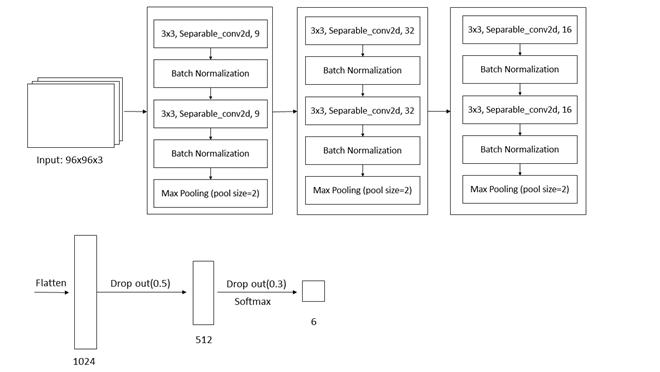
\includegraphics[width=\linewidth]{images/ktmang.png}
    \caption{ Minh họa kiến trúc mạng đã xây dựng}
    \label{fig:kientrucmang}
\end{figure}
% Do chip nhúng gì đó chỉ có bao nhiêu ram đó nên chúng tôi không thể xây dựng mô hình với trong số quá lớn và có chi phí tính toán cao được, nên chúng tôi sử dụng ...(thêm đoạn sau vô nè)
% Thêm dụ giảm kích thước của hình ảnh từ bao nhiêu đó xuống 96 * 96 nữa nà
Sử dụng separable convolution thay cho lớp convolution thông thường để giảm bớt chi phí tính toán cho mạng. Ngoài ra ở lớp này, chúng tôi dùng regularization l2 để tránh overfitting và hàm kích hoạt relu – đây là hàm thường được sử dụng trong quá trình train model với dữ liệu dưới dạng ảnh. Chúng tôi cũng thêm các lớp batch normalization và drop out để tránh cho mô hình bị overfitting và loại bỏ sự kết nối chặt chẽ giữa các lớp fully connected. Tổng số tham số của mô hình là 532,161. Sau khi xây dụng mô hình, nhóm đã sử dụng optimization stochastic gradient descent với learning rate = 1e-4 và momentum = 0.8 để train mô hình.

\section{Evaluation}
\subsection{Data Description} % Giới thiệu về dataset ddùng để train và test 
% Dữ liệu được lấy từ cái gì đó quên oy, nhưng cái này nên thêm vô nha
% Kích thước của hình là ... không nhớ a
Gồm 2527 hình thuộc 6 lớp với sự phận bố ở mỗi lớp:
 
Cardboard: 403

Glass: 501

Metal: 410

Paper: 594

Plastic: 482

Trash: 137
 
Dữ liệu được chia làm 2 phần theo tỉ lệ 80\% train và 20\% test.

Train: 2024

Test: 503
% Nên lựa vài hình về data để thêm vô (nếu cần) hình nên có đủ 6 lớp cần phân loại
\subsection{Index of Performance} % Các chỉ số để dánh gia model  %accuracy, F-score - Recall.
Chúng tôi sử dụng hai chỉ số là accuracy và F1-score để đánh giá model. Accuracy là tính tỉ lệ giữa số ảnh được dự đoán đúng và tổng số ảnh trong tập dữ liệu kiểm thử.
% Còn khúc giới thiệu F1 nữa cơ mà đang lười ghi công thức toán trong đây nha
% Khúc này thêm lý thuyết của hai cái chỉ số đó
\subsection{Results} % Kết quả  hiện thực được 
Kết quả train mô hình với 80 epoch
\begin{figure}[ht]
    \centering
    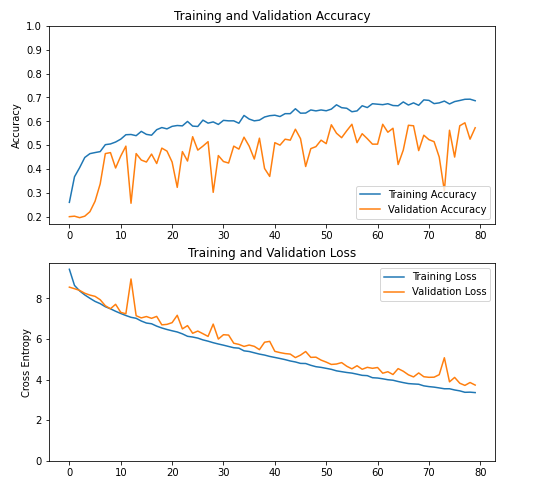
\includegraphics[width=\linewidth]{images/graph.png}
    \caption{ Biểu đồ thể hiện loss và accuracy của mô hình trong quá trình train}
    \label{fig:graph}
\end{figure}
% Hai cái này nên chuyển thành dạng bảng, cơ mà đang lười chuyển
Accuracy cao nhất trên tập train là 0.6938 và trên tập test là 0.5938
Loss nhỏ nhất trên tập train là 3.3844 và trên tập test là 3.7116

Kết quả thử nghiệm mô hình trên tập test sau khi đã lưu mô hình tốt nhất từ quá trình train 
\begin{figure}[ht]
    \centering
    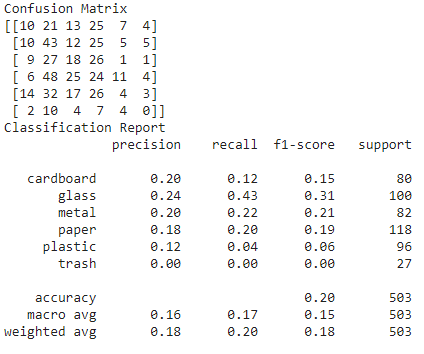
\includegraphics[width=\linewidth]{images/matrix.png}
    \caption{ Confusion matrix của model khi thử lại trên tập test}
    \label{fig:matrix}
\end{figure}
Từ hình \ref{fig:matrix} ta có thể thấy accuracy và f1-score của mô hình còn khá thấp, tuy nhiên do mô hình được xây dựng chỉ có 532,161 tham số nên không đủ để phân loại chính xác các lớp được. Chúng tôi đã thử train thêm epoch nhưng mô hình dễ bị overfitting và kết quả khi in confusion matrix vẫn không thay đổi nhiều. Ngoài ra nếu tăng thêm trọng số thì không thể sử dụng model trên thiết bị được.

\include{Chapter4/Chapter4}
% !TEX root = ..\thesis.tex



\chapter{THIẾT BỊ}
\label{chap:application}

\section{Giới thiệu mạch ESP32 CAM AI THINKER}

\section{Giới thiệu mạch ESP32 Heltech}

\section{Giới thiệu gateway Dragino LN-02}





% % !TEX root = ..\thesis.tex
\nheading{TÀI LIỆU THAM KHẢO}

\begin{thebibliography}{99}

\bibitem{DBPedia} Bizer, Christian, Jens Lehmann, Georgi Kobilarov, Sören Auer, Christian Becker, Richard Cyganiak, and Sebastian Hellmann. "DBpedia-A crystallization point for the Web of Data." Web Semantics: science, services and agents on the world wide web 7, no. 3 (2009): 154-165.

\bibitem{trashnet} Gary Thung, Mindy Yang, "TrashNet dataset"


\end{thebibliography}
% \printbibliography

\begin{thebibliography}{SJL05}

\bibitem{trashnet} Gary Thung, Mindy Yang. \textit{Classification of trash for recyclability status}.CS229 Project Report2016, 2016.

\bibitem{DBPedia} Bizer, Christian, Jens Lehmann, Georgi Kobilarov, Sören Auer, Christian Becker, Richard Cyganiak, and Sebastian Hellmann. "DBpedia-A crystallization point for the Web of Data." Web Semantics: science, services and agents on the world wide web 7, no. 3 (2009): 154-165.
    

\end{thebibliography}

\end{document}
